
\chapter{概述}
\section{交通信号控制概述}
交通信号控制是一个重要而具有挑战性的现实问题,其目的是通过协调车辆在道路交叉口的运动来最小化所有车辆的通行时间。目前广泛使用的交通信号控制系统仍然严重依赖过于简化的信息和基于规则的方法。车联网技术的发展、硬件性能的提升以及人工智能技术的进步使得我们现在有更丰富的数据、更多的计算能力和先进的方法来驱动智能交通的发展。 
交通信号控制的目的为了方便车辆在交叉路口的安全和高效移动。安全是通过信号灯指定不同车道的车通行来分离相互冲突的运动实现的。为了能够有效地优化通行效率,已有的工作提出了不同的指标来量化通行效率,主要有以下三个:
\begin{itemize}
    \item 通行时间:在交通信号控制中,车辆的行驶时间被定义为一辆汽车进入系统的时间与离开系统的时间的差值。 最常见的优化目标之一是就是减少进过路口的所有车辆的平均通行时间。
    \item 队列长度:队列长度是指路口等待车辆的数量,越大的队列长度意味着越多的等待车辆,路口的通行效率越低,反之通行效率越高。
    \item 路口吞吐量:吞吐量是指在一定期间内进过路口完成通行的车辆数量。越大的吞吐量代表着越高的通行效率,所以很多工作将最大化吞吐量作为优化的目标。
\end{itemize}

\begin{figure}[htb]
    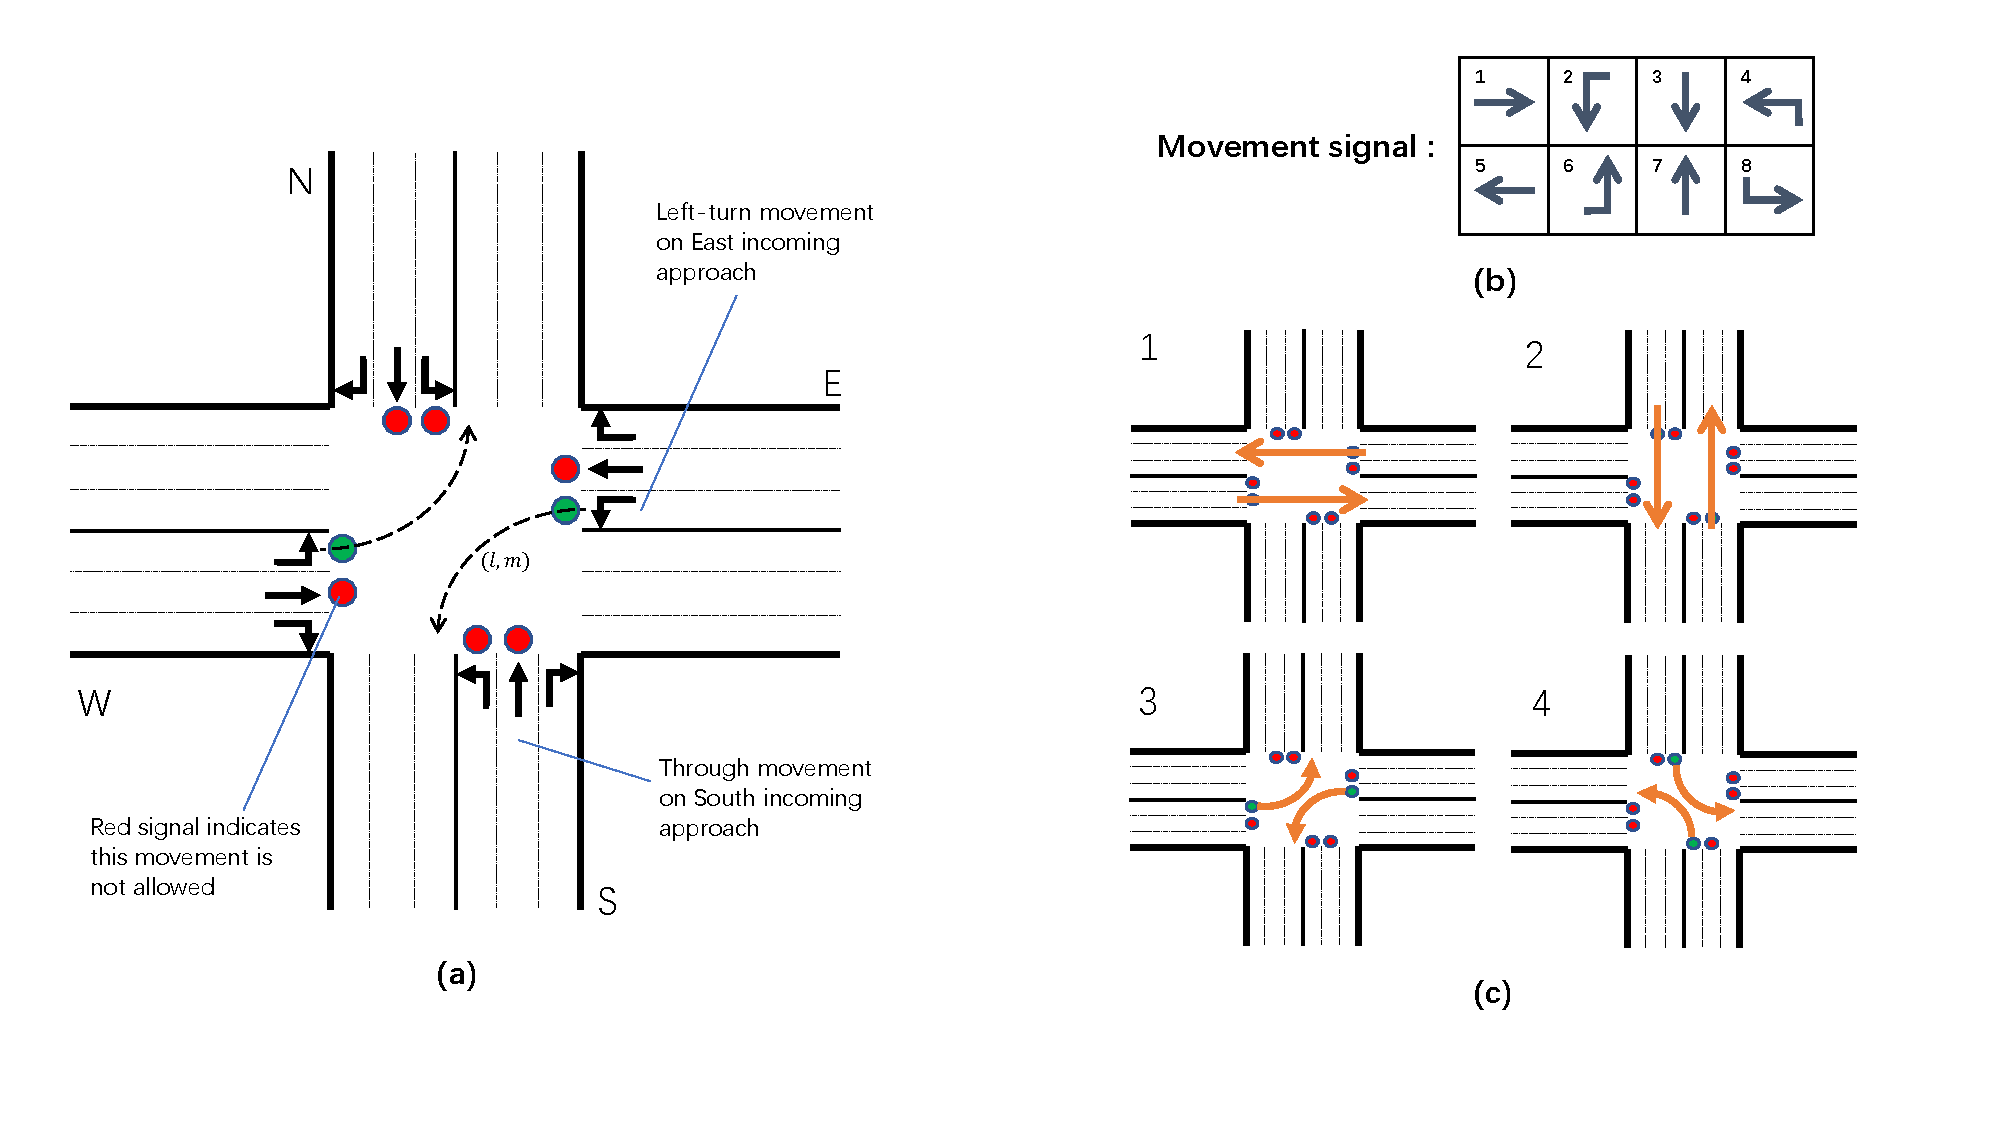
\includegraphics[width=.9\textwidth]{fig/tsc.pdf}
    \caption{交通信号术语图示}
    \label{fig:tsc}
\end{figure}
\subsection{基本术语}
\begin{itemize}
    \item Approach: 指交叉路口的巷道。任何一个交叉路口都有两种approach,即转入巷道(incoming approach)和转出巷道(outgoing approach)。\autoref{fig:tsc}(a)描述了一个典型的有8个approach(四个转入巷道,四个转出巷道)的交叉路口。
    \item Lane:一个Approach是由一组车道组成。与Approach的定义类似,车道也分为两种:转入车道(incoming lane)和转出车道(outgoing lane)。
    \item Traffic movement:指的是车流从一个incoming approach 运动到另一个outgoing approach,表示为$\left(r_{i}, r_{o}\right)$,其中ri和ro分别表示incoming lane和outgoing lane。通常,traffic movement可以分为左转、直行以及右转三种,在少数特殊的路口也支持U-turn的traffic movement。
    \item Movement signal:根据traffic movement定义的运动信号,绿色代表可以通行,红色代表禁止通行。根据大多数国家的交通规则,右转的traffic movement是可以不受信号约束的。
    \item Phase: 信号灯的一个phase(相位)是指非冲突运动信号的组合,这意味着这些信号可以同时设置为绿色,而不会引起安全冲突。 \autoref{fig:tsc}(c)展示了最常用的四相位信号模式。
    \item Phase sequence: 相序,即一组信号相位的序列,它定义了一组信号相位及其变化顺序。
    \item Signal plan:信号计划,由一组相位序列及其相应的起始时间组成。通常表示为$\left(p_{1}, t_{1}\right)\left(p_{2}, t_{2}\right) \ldots\left(p_{i}, t_{i}\right) \ldots$其中$p_{i}$ 和 $t_{i}$分别代表相位及其开始时间。
    \item Cycle-based signal plan:周期性信号计划,与普通的信号计划不同的是其中的相位序列是按循环顺序工作的,可以表示为
    $\left(p_{1}, t_{1}^{1}\right)\left(p_{2}, t_{2}^{1}\right) \ldots \\ \left(p_{N}, t_{N}^{1}\right)\left(p_{1}, t_{1}^{2}\right)\left(p_{2}, t_{2}^{2}\right) \ldots\left(p_{N}, t_{N}^{2}\right) \ldots$,其中$p_{1}, p_{2}, \ldots, p_{N}$是重复出现的相位序列,$t_i^j$是$j$周期中相位$p_i$的起始时间。具体地,$C^{j}=t_{1}^{j+1}-t_{1}^{j}$是第j周期的周期长度, $\left\{\frac{t_{2}^j-t_{1}^j}{C^j}, \ldots, \frac{t_{N}^j-t_{N-1}^j}{C^j}\right\}$是第$j$周期中的相位分裂比(phase split ratio),表示每个相位持续时间占总周期长度的比重。现有的交通信号控制方法通常在一天中重复类似的相位序列。
\end{itemize}


\section{传统交通信号控制方法}
\subsection{Fixed-Time}
使用最为广泛的一种交通信号控制方法,按照事先固定的信号序列不断的循环,不依赖于任何类型的检测,例如行人按钮或车辆检测装置。所有道路和运动都以恒定的特定顺序提供服务。即使没有汽车或行人,信号也会改变,在交通较为稳定的情况下能够起到不错的效果,但是当交通变化很大时效率会很低。由于不需要安装任何检测器,所以这种方法的成本效益高。

\subsection{Webster}
Webster方法是一种广泛使用的针对单路口场景的交通信号控制方法。对于单路口场景,传统交通信号控制方法通常由三个部分组成:确定信号周期长度,确定信号相位序列以及相位分裂。Webster的做法就是根据交通流量计算信号周期长度和相位分裂时间。通过假设车流在一段时间内(例如,过去的五分钟或10分钟)是均匀到达的,可以计算出确切的最优周期长度和最佳相位分裂时间,从而最小化车辆通行时间。周期长度计算依赖于以下方程:
\begin{align}
    C_{d e s}\left(V_{c}\right)=\frac{N \times t_{L}}{1-\frac{V_{c}}{\frac{3600}{h} \times P H F \times(v / c)}}
\end{align}
其中$N$是信号相位的数量(既有多少种不同的信号相位),$t_{L}$是每个相位下的总共延误时间,可以看作是一个与全红信号相位(全是红灯,所有的交通都不允许通行)时间以及车辆的加减速相关的参数。参数$h$则是饱和间隔时间(单位:秒/车),指前后车辆通过道路上某一点的最小时间间隔。$PHF$是一个交通高峰时段因子,是衡量高峰时段交通需求波动的参数。$v / c$是期望的流量与容量比,用来描述路口的繁忙程度。这些参数在不同的交通条件下会有不同的值,通常是根据经验观察和机构标准来选择。
在确定周期长度后就可以算出绿色信号比(即在一个周期时间内,绿色信号所占的时间比重),具体计算方式如下:
\begin{align}
    \frac{t_{i}}{t_{j}}=\frac{V_{c}^{i}}{V_{c}^{j}}
\end{align}
$t_i \text{和} t_j$分别表示相位$i$和相位$j$的时长。$V_c^i$表示相位$i$的临界车道流量,其中临界车道是指在一个相位中交通流量与饱和流量之比最高的车道,通常与队列长度有关。

\subsubsection{MaxBand}
MaxBand是一种以优化邻居路口的通行效率为目标的传统交通信号调度算法,与GreenWave不同的是,它旨在根据整个路网系统内各个路口的信号计划找到一个最大的带宽(maximal bandwidth )来减少沿两个相反方向行驶的车辆的停靠次数。
其中带宽是指同步绿波在一个周期长度内所持续的部分时间,通常较大的带宽意味着沿一个方向的更多交通可以不间断地通过。与GreenWave相同的是,MaxBand同样要求所有路口具有相同的信号周期长度(通常设置为所有信号周期长度最大值)。在遵循以下约束条件的情况下,MaxBand会通过使用一个混合整数线性规模模型来计算出一个对称且宽度统一的带宽。
\begin{itemize}
    \item 单个路口的带宽限制:首先对于每个方向(包括入站方向和出站方向,入站方向指的是进入交叉路口的方向,出战方向则是离开交叉路口的方向)来说,绿色信号的时间应该大于带宽的长度:
    \begin{align}
        \label{eq:band-cons-1}
        w_i + b \leq 1- r_i, w_i > 0,
    \end{align}
    \begin{align}
        \label{eq:band-cons-2}
        \hat{w_i} + \hat{b} \leq 1- \hat{r_i}, w_i > 0,
    \end{align}
    这里$w_i \text{和} \hat{w-i}$分别表示入站和出站方向上红色信号结束可带宽开始之间的时间间隔,$b$值得是带宽,$r_i \text{和} \hat{r_i}$分别表示入站和出站方向的红色信号时间。
    其次对于两个不同的方向,入站和出战的带宽要相同:
    \begin{align}
        \label{eq:band-cons-3}
        b = \hat{b}
    \end{align}
    \item 路口$i$和路口$j$之间时间和空间的偏移量约束:首先时间上要满足下列约束条件:
    \begin{align}
        \label{eq:temporal-cons}
        \theta(i,j) + \hat{\theta}(i,j) + \delta_i - \delta_j = m(i,j),
    \end{align}
    这里$\theta(i,j)¥\textbf{和}\hat{\theta}(i,j)$分别表示路口入站和出站的偏移量,$\delta$ 为入站和出站的红色信号时间偏移量,$m(i,j)$是一个整数变量,表示路口$i$和路口$j$的信号周期长度的一个倍数。
    其次空间上,车辆从一个路口出发到另一个路口的行驶时间要满足以下约束条件:
    \begin{align}
        \label{eq:spataril-cons-1}
        \phi(i, j)+0.5 * r_{j}+w_{j}+\tau_{j}=0.5 * r_{i}+w_{i}+t(i, j),
    \end{align}

    \begin{align}
        \label{eq:spataril-cons-2}
        \hat{\phi}(i, j)+0.5 * \hat{r}_{j}+\hat{w}_{j}=0.5 * \hat{r}_{i}+\hat{w}_{i}-\hat{\tau}_{i}+\hat{t}(i, j)
    \end{align}
    其中$t$和$\hat{t}$分别表示交叉路口之间的进站和出战的通行时间,与道路的长度和车辆行驶速度有关;$\tau \text{和} \hat{\tau}$表示交叉路口的队列清理时间,与从其他路口转入以及自身的交通流量有关。
\end{itemize}
最后MaxBnad的优化目标定义如下所示:
\begin{equation}
    \begin{split}
        \textbf { maximize } b \\
        \textbf { subject to } \text { \ref{eq:band-cons-1}, \ref{eq:band-cons-2}, \ref{eq:band-cons-3}, \ref{eq:temporal-cons}, \ref{eq:spataril-cons-1}, \ref{eq:spataril-cons-2}} \\
        {m_{i} \in \mathbb{N}} \\
        {b, \bar{b}, w_{i}, \bar{w}_{i} \geq 0, i=1, \ldots, n}.
    \end{split}
\end{equation}

\subsection{GreenWave}
虽然使用Webster可以简单的控制单个交叉路口的交通信号,但是对于相邻的多个交叉路口,不能够简单地直接使用Webster来分别优化每一个路口,相邻路口信号灯的信号时间之间的偏移(即相邻路口信号周期起始时间的差值)也需要进行优化,因为对于相距较近的路口来说,一个路口的控制策略可能会影响到其他路口。
GreenWave就是交通运输领域中最经典的协调相邻路口的信号控制方法,它通过优化相邻路口信号时间的偏移来减少车辆在某一方向行驶时的停留次数。其中路口之间的偏移量通过以下公式计算:
\begin{align}
    \label{eq:green-wave}
    \Delta t_{i, j}=\frac{L_{i, j}}{v}
\end{align}
其中$L_{i, j}$是路口$i$和路口$j$之间的道路长度,$v$是道路上车辆的预期行驶速度。这种方法可以形成沿指定交通方向的绿色信号波,在该方向行驶的车辆可以受益于渐进的绿色信号级联,而不会在任何交叉口停留,如图\autoref{fig:green-wave}所示:
\begin{figure}[htb]
    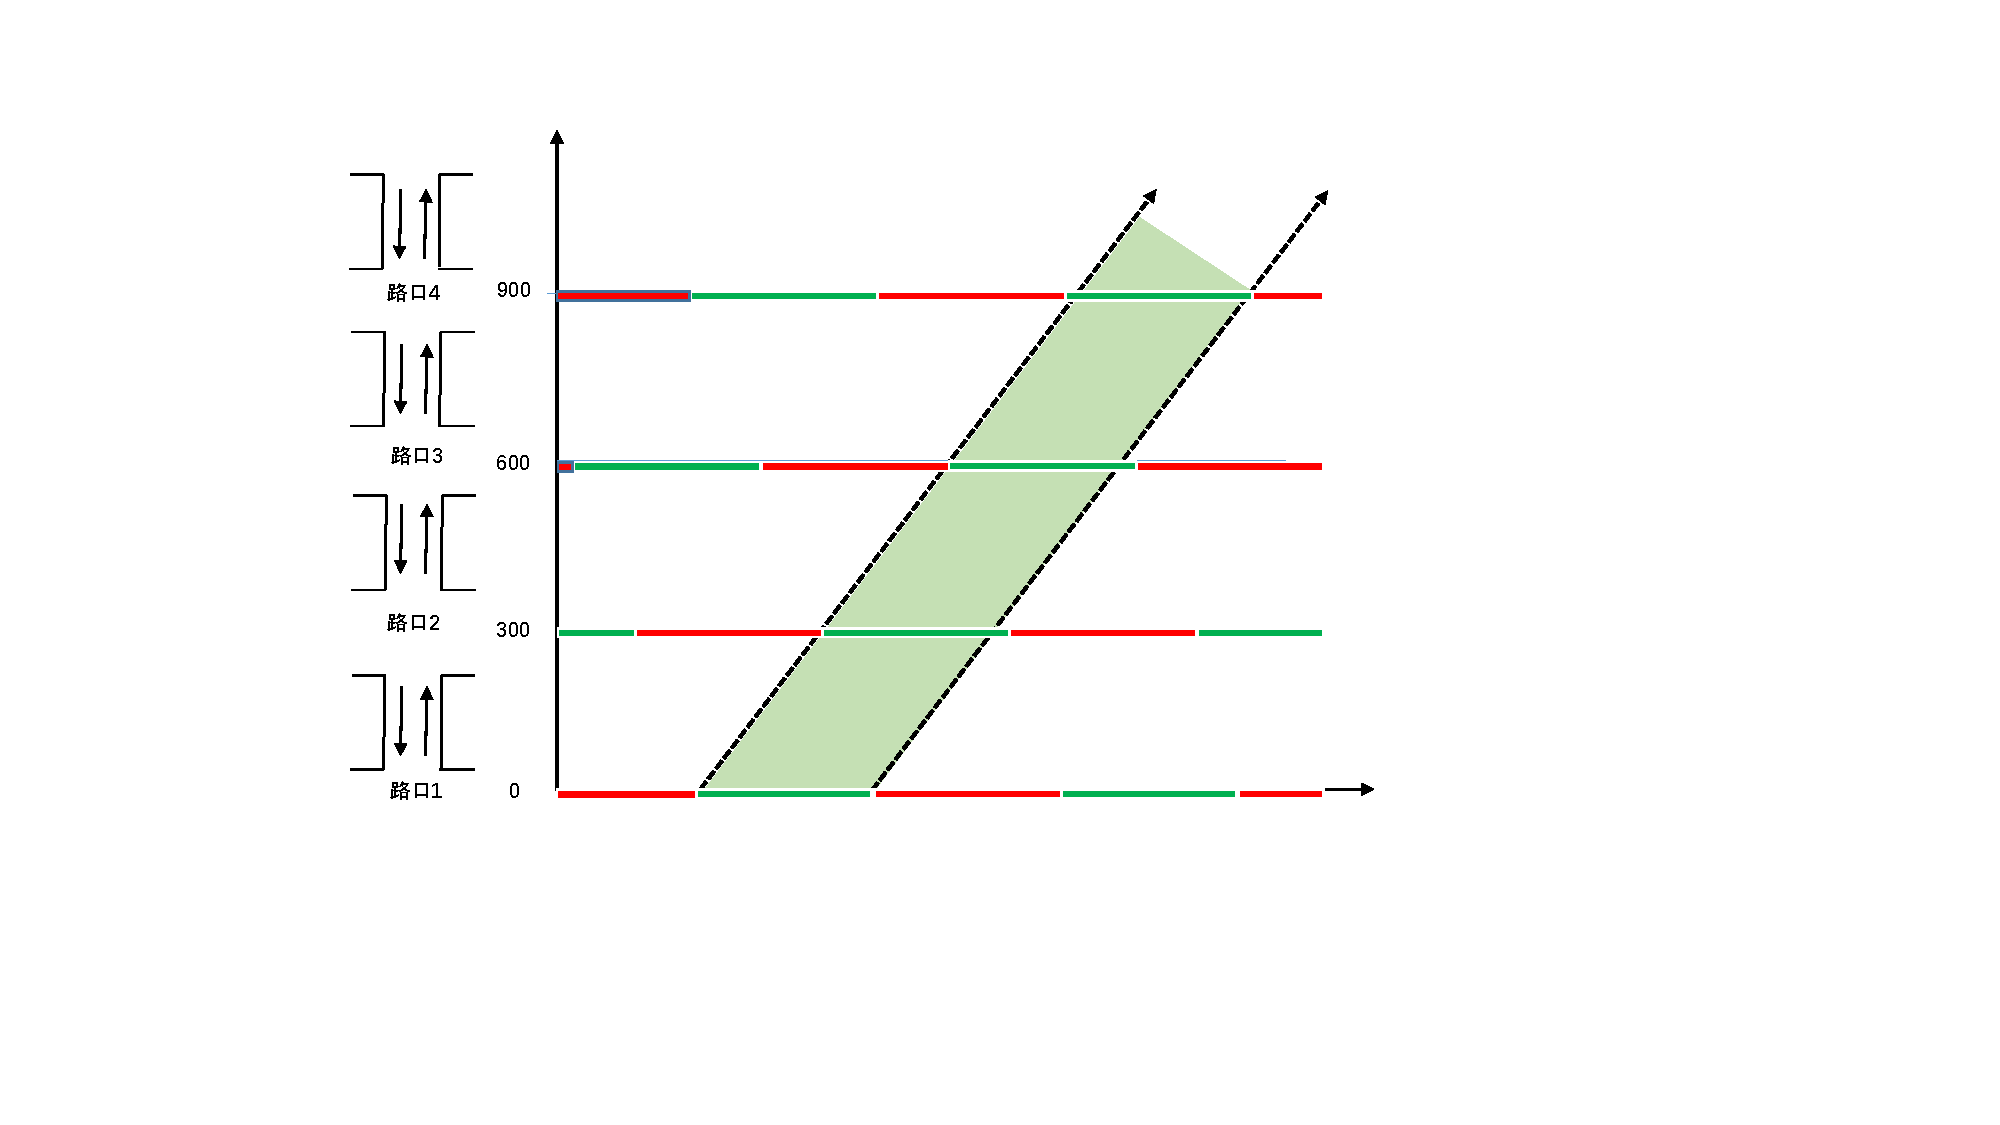
\includegraphics[width=1.2\textwidth]{fig/green-ware.pdf}
    \caption{GreenWave方法的绿色信号波示意图}
    \label{fig:green-wave}
\end{figure}

\subsection{Actuated Control}
Actuated Control根据当前信号相位和其他的竞争信号相位对绿色信号的请求来决定是否保持或者变化当前的相位,根据规则的差异,Actuated Control主要可以分为Fully-Actuated Control和Semi-Actuated Control两种。具体的请求触发规则定义如\autoref{tab:actuated-control}所示:
\begin{table}[htb]
    \caption{Actuated Control 信号相位请求触发规则\label{tab:actuated-control}}
    \begin{tabular}{ccl}
      \toprule
      \tabincell{l}{来自当前信号\\相位的请求} & \tabincell{l}{来自其他信号\\相位的请求} & \tabincell{c}{动作} \\
      \midrule
      \multirow{2}{*}{是} & 是 & \tabincell{l}{\textbf{Fully-actuated control}:如果当前信号相位的持续时间大于阈值,\\则切换到下一信号相位;否则,保持当前信号相位。\\\textbf{Semi-actuated control}:保持当前信号相位。 } \\
      \cline{2-3}                    
      & 否 & 保持当前信号相位。\\
      \hline
      \multirow{2}{*}{否} & 是 & 切换到下一信号相位。\\
      \cline{2-3}
                          & 否 & \tabincell{l}{\textbf{Fully-actuated}:保持当前信号相位。\\\textbf{Semi-actuated control}:切换到默认信号相位(通常\\设置为主干道的绿色信号)。}\\
      \\
      \bottomrule
    \end{tabular}
\end{table}


\subsection{SOTL}
SOTL(Self-Organizing Traffic Light Control)是一种具有附加需求响应规则的Fully-Actuated Control方法。它与Fully-Actuated Control的主要区别在于当前信号相位的绿色信号请求定义(虽然它们都需要最小的绿色相位持续时间),在Fully-Actuated Control中,当车辆接近信号灯时,就会产生延长绿色信号的请求,而在SOTL中,除非接近信号灯的车辆数量大于预先定义的一个阈值,否则就不会产生绿色信号请求。

\subsection{Max-Pressure Control}
Max-Pressure Control的目的是通过最小化对应信号相位的压力(pressure)来平衡相邻路口之间的队列长度,从而降低过饱和的风险,其中压力的概念如图\autoref{fig:max-pressure}所示:
\begin{figure}[htb]
    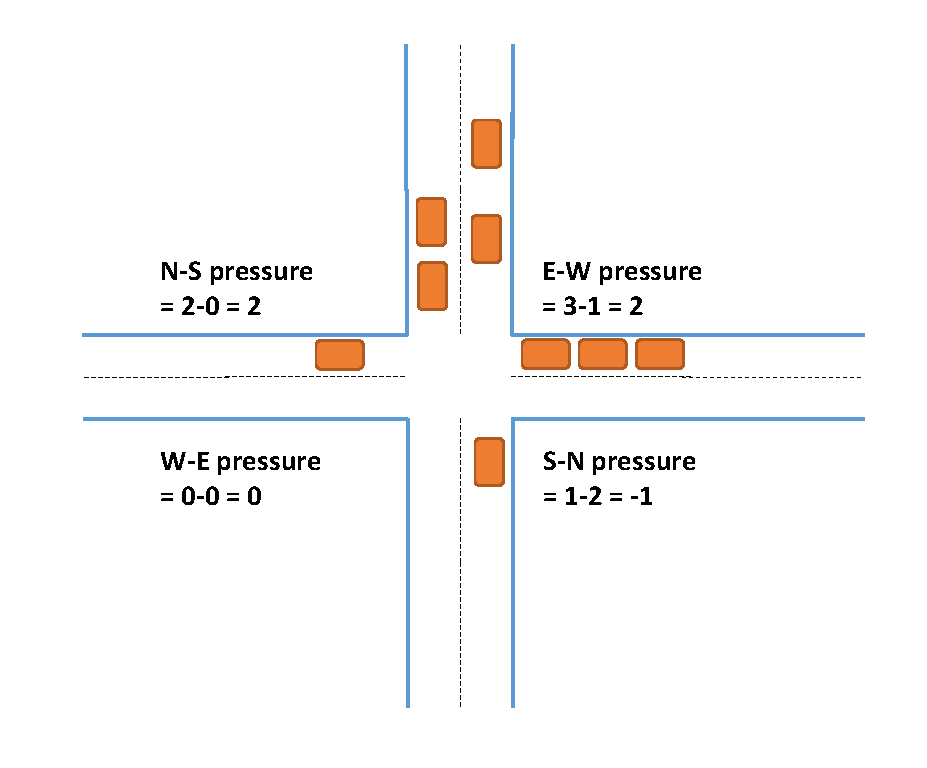
\includegraphics[width=0.9\textwidth]{fig/max-pressure.pdf}
    \caption{Max-Pressure的压力图示}
    \label{fig:max-pressure}
\end{figure}
其中运动信号的压力是指转入车道上的车辆数减去相应的转出车道上的车辆数,而信号相位的压力定义为转入巷道和转出巷道上的总队列长度之间的差异。Varaiya\cite{varaiya2013max}等人证明了当将优化目标设为最小化单个路口的相位压力时,Max-Pressure Control可以最大限度地提高真个路网的吞吐量。Max-Pressure Control算法流程如\autoref{alg:max-pressure-alg}所示:
\begin{breakablealgorithm}
    \caption{Max-Pressure Control算法流程}
    \label{alg:max-pressure-alg}
    \begin{algorithmic}[1] %每行显示行号  
        \Require 
        $t$ : 当前信号相位时间。\\
        $t_{min}$ :最小信号相位持续时间。 

        \For{\textbf{all} timestamp}
        \State $t = t+1$。
        \If{$ t \geq t_{min}$}
        \State 计算每个信号相位 $i$ 的压力 $P_i$。
        \State 选择压力最大的信号相位 $i=\mathop{\arg\max}_i{P_i}$。
        \State 重置信号时间 $t=0$。
        \EndIf
        \EndFor
    \end{algorithmic}  
\end{breakablealgorithm}  

\subsection{SCATS}
SCATS通过将预先定义的信号计划(包括信号周期长度、信号相位分裂比以及偏移量)作为输入,并根据事先定义的性能指标来从这些反复选择,其性能指标饱和度的定义如下:
\begin{align}
    D S=\frac{g_E}{g}=\frac{g-\left(h^{\prime}-h \times n\right)}{g}
\end{align}
其中$g$是可用的绿色信号时间,$g_E$是有车辆通过路口的有效绿色信号时间,等于可用绿色信号时间减去浪费的绿色信号时间,而浪费的绿色信号时间是通过检测来计算的,$h^{\prime}$是检测到的总时间差,$n$是检测到的车辆数量,$h$是车辆之间的单位饱和间隔,它表示连续车辆通过一个点的最小时间间隔。
信号相位分裂比、信号周期长度以及偏移量是通过近似机制从实现定义的信号计划中选择的。以信号相位分裂比的选择为例,SCATS首先计算当前信号计划下的饱和度,然后使用以下公式估计出在当前信号周期内为被应用的其他信号计划的饱和度。
\begin{align}
    \hat{D S^j_p} = \frac{D S_p \times g_p}{g_p^j}
\end{align}
其中$D S_p\text{和} g_p$分别是信号相位$p$在当前信号计划下的饱和度以及绿色信号时间,$g^j_p$是信号相位$p$在信号计划$j$下的饱和度,具体的算法流程如\autoref{alg:scats}所示。
\begin{breakablealgorithm}
    \caption{SCATS中信号相位分裂比的选择算法流程}
    \label{alg:scats}
    \begin{algorithmic}[1] %每行显示行号  
        \Require 
        $A={a_j|j=1,2,\cdots,N}$ : 候选的信号计划集合\\
        $a_c$ :当前的信号计划。 
        \For{textbf{all} $p in {1, \cdots, P}$} 
            \State 计算每个信号相位$p\in{1,\cdots, P}$在当前信号计划$a_c$下的饱和度$D S_{p}$。
        \EndFor
        \For{textbf{all} $a_j$ in $A$}
            \State 计算每个信号相位$p$在信号计划$a_j$下的饱和度$\hat{D S^j_p}$。
        \EndFor
    \end{algorithmic}  
\end{breakablealgorithm}  

\autoref{tab:traditional-methods}列出了每种方法的要求和输出结果:
\begin{table}[htb]
    \caption{传统交通信号控制方法总结\label{tab:traditional-methods}}
    \begin{tabular}{llll}
      \toprule
      方法 & 先验信息 & 输入 & 输出 \\
      \midrule
      Webster & 相位序列 & 交通流量 & 基于周期的单个路口信号计划 \\
      \hline
      \tabincell{l}{GreenWave\\MaxBand} & 信号计划 & \tabincell{l}{交通流量\\速度限制\\车道长度} & 基于周期的信号计划的偏移量 \\
      \hline
      \tabincell{l}{Actual Control\\SOTL} & 相位序列& 交通流量 & 是否变化到下一个相位\\
      \hline
      Max-Pressure Control & 无 & 队列长度 & 所有交叉口的信号计划\\
      \hline
      SCATS & 所有路口信号计划 & 交通流量 & 调整后的信号计划\\
      \bottomrule
    \end{tabular}
\end{table}

\section{基于强化学习的交通信号控制}
最近,人们提出了不同的人工智能技术来控制交通信号,例如遗传算法、群体智能以及强化学习(Reinforcement Learning,RL)。 其中在这些技术中,强化学习在近年来更具趋势。
\subsection{强化学习概述}
\begin{figure}[htb]
    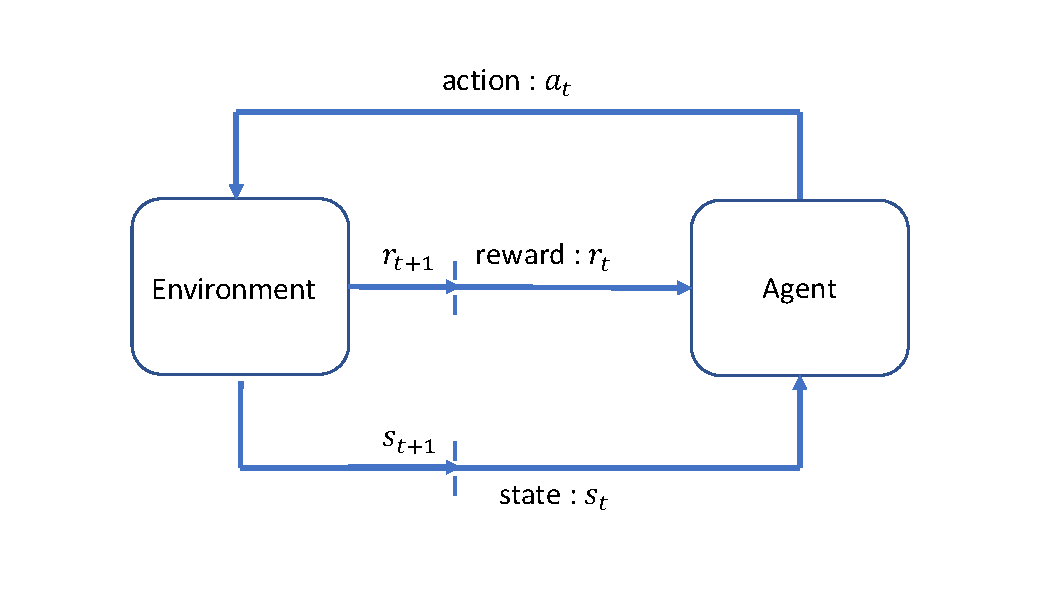
\includegraphics[width=0.9\textwidth]{fig/rl.pdf}
    \caption{马尔可夫决策过程示意图}
    \label{fig:mdp}
\end{figure}
通常单智能体强化学习问题被建模成马尔可夫决策过程(Markov Decision Process, MDP, 如\autoref{fig:mdp}所示) $<\mathcal{S}, \mathcal{A}, P, R, \gamma>$,其中$\mathcal{S}, \mathcal{A}, P, R, \gamma$分别表示状态集、动作集、状态转移函数、奖励函数和折扣因子。具体定义如下:
\begin{itemize}
    \item $\mathcal{S}$:在时间步骤$t$,智能体得到一个观测状态$s^t \in \mathcal{S}$。
    \item $\mathcal{A}, P$:在时间步骤$t$,智能体采取一个动作$a^t \in \mathcal{A}$,然后环境根据状态转移函数转移到一个新的状态。
    \begin{align}
        P\left(\mathrm{~s}^{t+1} \mid \mathrm{s}^{t}, \mathrm{a}^{t}\right): \mathcal{S} \times \mathcal{A} \rightarrow \mathcal{S}
    \end{align}
    \item $R$:在时间步骤$t$,智能体通过奖励函数获得一个奖励$r^t$。
    \begin{align}
        R\left(s^{t}, a^{t}\right): \mathcal{S} \times \mathcal{A} \rightarrow \mathbb{R}
    \end{align}
    \item $\gamma$:智能体的目标是找到一种使预期收益最大化的策略,即累积(折扣)奖励之和。折扣因子决定了即时奖励与未来奖励的重要性。
    \begin{align}
        G^{t}:=\sum_{i=0}^{\infty} \gamma^{i} r^{t+i}
    \end{align}
  \end{itemize}
    解决一个强化学习任务意味着要找到一个能够使预期收益最大化的最优策略$\pi^*$,一般来说,我们难以直接找到这个最优策略,更多的是比较若干个不同的策略然后从中选出较好的那个作为局部最优解。而策略的筛选是通过比较其对应的价值函数来实现的,即通过寻找较优的价值函数来筛选出较优的策略。价值函数是对未来奖励的期望,根据输入的不同可以分为状态价值函数和动作价值函数。
状态价值函数的定义如下:
\begin{align}
    V_{\pi}(s)=\mathbb{E}_{\pi}\left[G_{t} \mid S_{t}=s\right]
\end{align}
其描述的是当在$t$时刻处于状态$s$的预期收益。动作价值函数的定义如下:
\begin{align}
    Q_{\pi}(s, a)=\mathbb{E}_{\pi}\left[G_{t} \mid S_{t}=s, A_{t}=a\right]
\end{align}
其描述的是当在状态$s$下采取动作$a$的预期收益。

最优策略$\pi^{*}$对应的是最优状态价值函数和最优动作价值函数。最优状态价值函数定义为$V_{\pi}^*(s)=\mathcal{max}_{\pi}V^{\pi}(s)$,它满足以下贝尔曼最优方程:
\begin{align}
    V^{*}\left(\mathrm{~s}^{t}\right)=\max _{\mathrm{a}^{t} \in \mathcal{A}} \sum_{\mathrm{s}^{t+1} \in \mathcal{S}} P\left(\mathrm{~s}^{t+1} \mid \mathrm{s}^{t}, \mathrm{a}^{t}\right)\left[\mathrm{r}+\gamma v_{*}\left(\mathrm{~s}^{t+1}\right)\right], \forall \mathrm{s}^{t} \in \mathcal{S}
\end{align}
最优动作价值函数定义为$Q^*(s,a)=\mathcal{max}_{\pi}Q^{\pi}(s,a)$,其满足以下贝尔曼最优方程:
\begin{align}
    Q^{*}\left(s^{t}, a^{t}\right)=\sum_{s^{t+1} \in \mathcal{S}} P\left(s^{t+1} \mid s^{t}, a^{t}\right)\left[r^{t}+\gamma \max _{a^{t+1}} Q^{*}\left(s^{t+1}, a^{t+1}\right)\right], \forall s^{t} \in \mathcal{S}, a^{t} \in \mathcal{A}
\end{align}

\subsubsection{分类}
\begin{figure}[htb]
    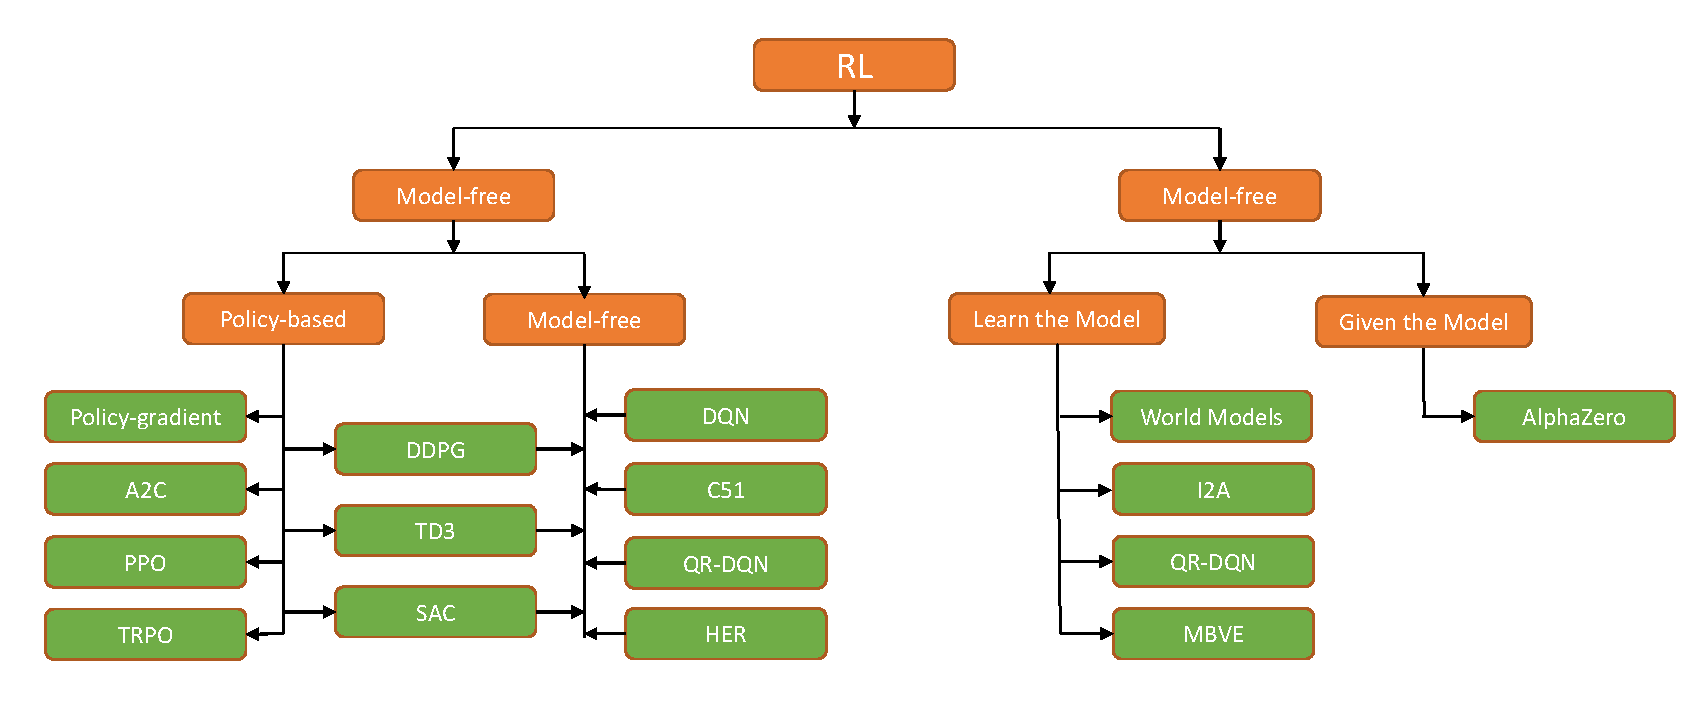
\includegraphics[width=0.9\textwidth]{fig/rl-classfication.pdf}
    \caption{强化学习分类及常见算法}
    \label{fig:rl-classficatoin}
\end{figure}
强化学习主要可以分为两大类:Model-based(有模型)和Model-free(无模型)。其中Model-based又可以分为基于策略函数(Policy-based)和值函数(Value-based)两大类,而Model-free可以分为模型学习(Learn the Model)和给定模型(Given the Model)两大类,具体如\autoref{fig:rl-classficatoin}所示。

Model-free方法是指在不知道状态转移函数函数的情况下,通过采样大量的经验来学习策略函数或者价值函数。其中Policy-based的方法直接将拟学习的策略参数化,在以最大化奖励的目标下,直接对策略函数进行优化。而Value-based的方法则是学习一个最佳策略对应的动作价值函数的近似。当然,Policy-based和Value-based并非无法兼容的,有一类方法(Actor-Critic)就是融合了两中方法的思想。
这类方法同时使用策略和价值评估来做出决策,其中,智能体会根据策略做出动作,而价值函数会对做出的动作给出评分,这样可以在原有的基于策略的方法的基础上加速学习过程,取得更好的效果。代表算法如\autoref{fig:rl-classficatoin}中的DDPG\cite{lillicrap2015continuous}、TD3\cite{fujimoto2018addressing}以及SAC\cite{haarnoja2018soft}等。

Model-based方法是指在已知状态转移函数的情况下,学习用一个模型去模拟环境,然后用这个模拟的环境去预测接下来可能会发生的所有所有情况并从中选择最有利的情况。

% 根据是否有学习环境模型可以分为:
% \begin{itemize}
%     \item Model-based:指在已知状态转移分布条件下,智能体根据这个模型做出预先设定好的决策。通常意义来讲,动态规划是一种有模型的强化学习算法。
%     \item Model-free:指在未知状态转移分布条件下,通过学习价值函数(Value Function)和策略函数(Policy Function)进行决策,通常需要大量的采样来估计状态、动作及反馈函数,从而优化动作策略。
% \end{itemize}
% 根据学习目标可以分为:
% \begin{itemize}
%     \item Value-based:这类方法的目标是学习价值函数,只能应用在不连续的、离散的环境下(如围棋或某些游戏领域),对于行为集合规模庞大、动作连续的场景(如机器人控制领域),其很难学习到较好的结果。代表算法有Q-learning\cite{watkins1992q},DQN\cite{mnih2015human}等。
%     \item Policy-based:这类方法直接对策略进行优化,使制定的策略能够获得最高的反馈。代表算法有Policy Gradient\cite{sutton2000policy}算法等。
%     \item Actor-Critic:这类方法同时使用策略和价值评估来做出决策,其中,智能体会根据策略做出动作,而价值函数会对做出的动作给出评分,这样可以在原有的基于策略的方法的基础上加速学习过程,取得更好的效果。代表算法有A2C\cite{barto1983neuronlike}等。
% \end{itemize}


\subsection{基于强化学习的交通信号控制框架}
\begin{figure}[t]
    \subfloat[单路口场景\label{fig:single-tsc-rl}]{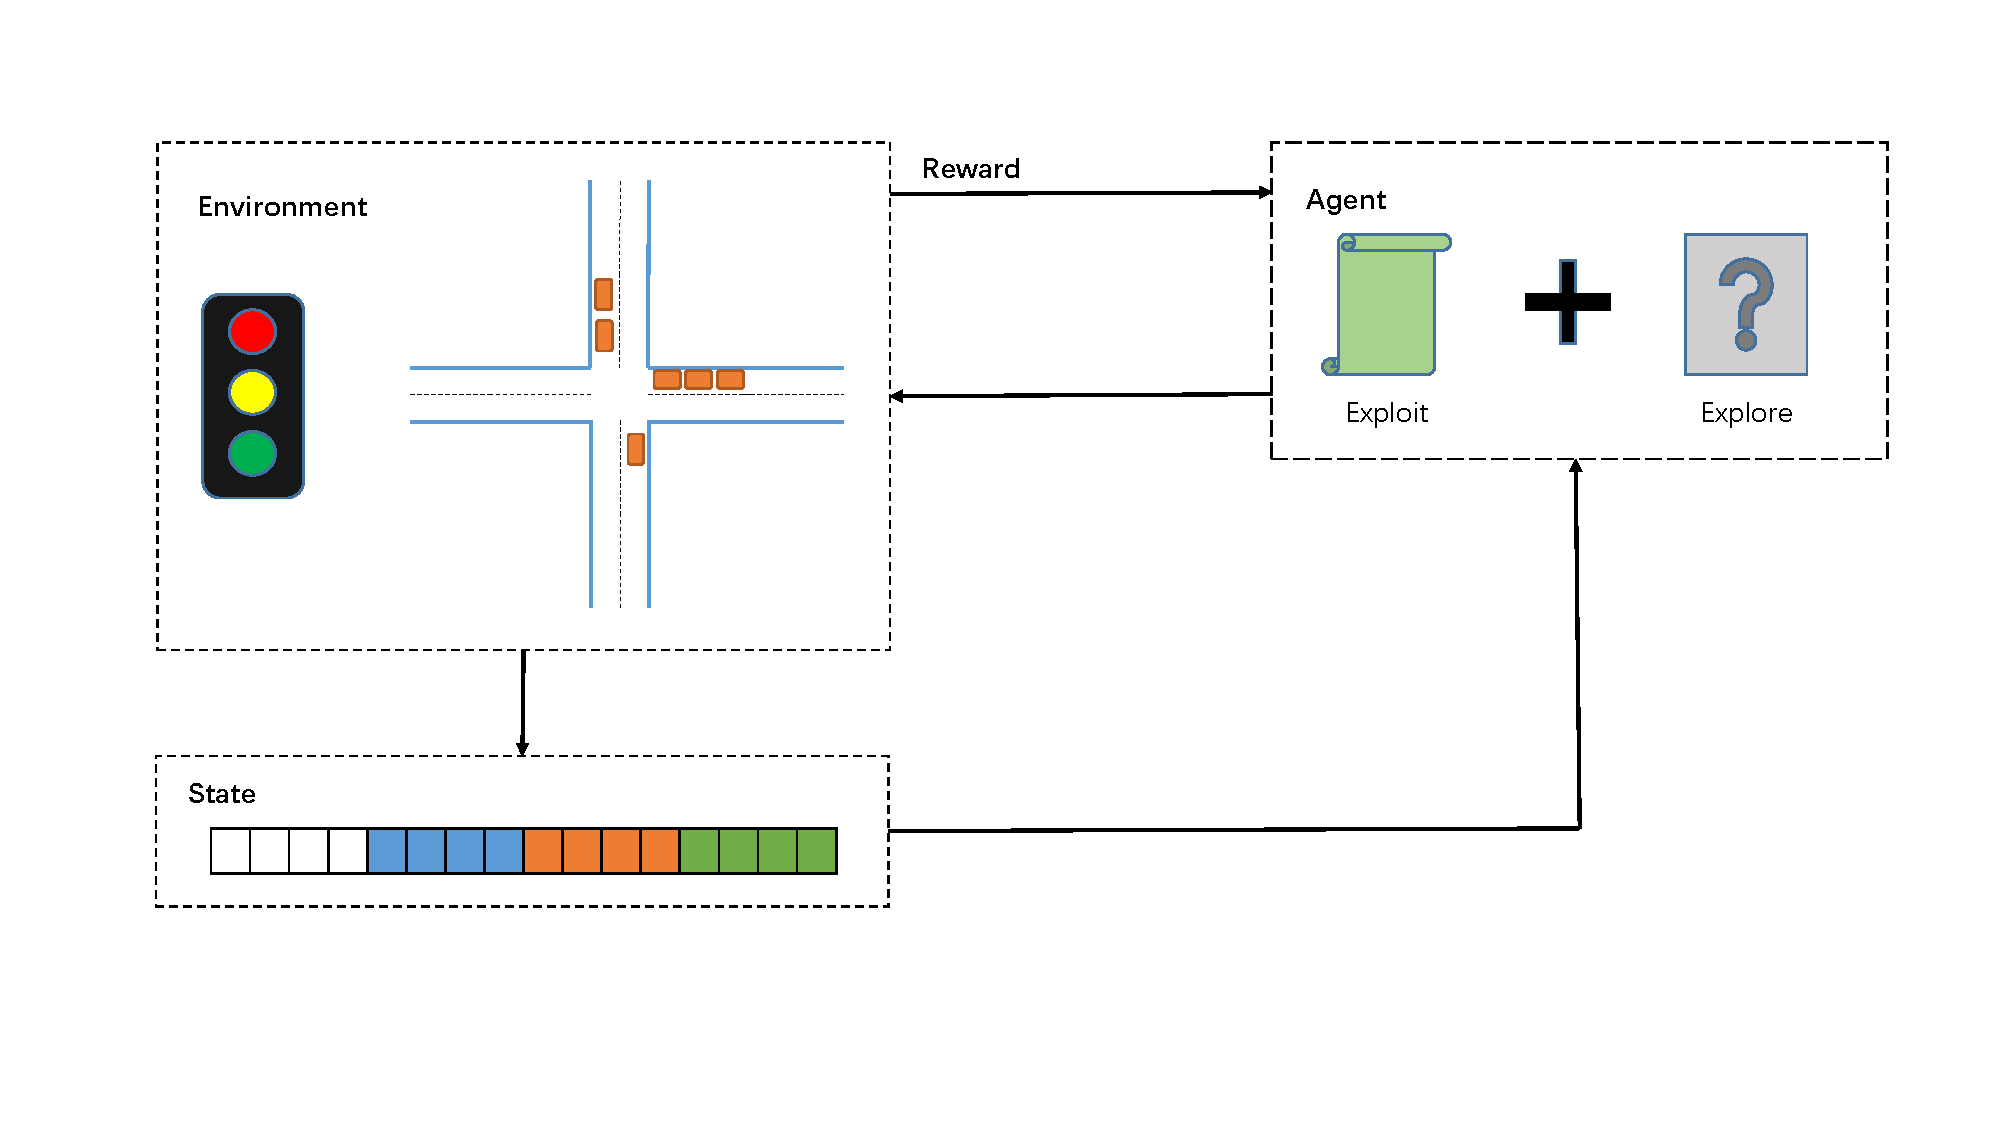
\includegraphics[width=0.45\textwidth]{./fig/single-intersection-RL.pdf}}\quad
    \subfloat[多路口场景\label{fig:multi-tsc-rl}]{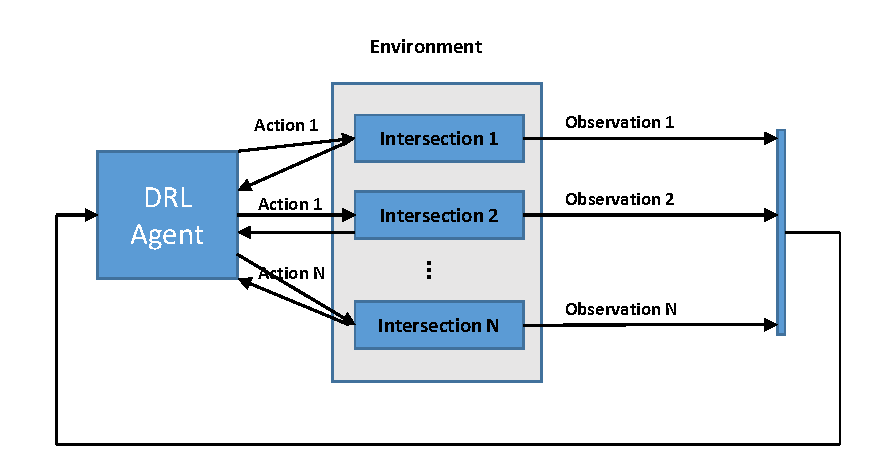
\includegraphics[width=0.45\textwidth]{./fig/multi-intersection-RL.pdf}}
    \caption{基于强化学习的交通信号控制框架}
    \label{fig:TSC-RL}
  \end{figure}
根据路网规模的不同,基于强化学习的交通信号控制框架可以分为以下两类:

\textbf{(1)基于深度强化学习的单路口交通信号控制框架}

\autoref{fig:TSC-RL}(a)描述了应用强化学习框架到单路口交通信号控制问题上的基本思路。环境是道路上的交通状况,智能体要做的是控制交通信号。在每个调度时刻$t$,获取环境的状态描述$s^t$(例如,当前的信号相位,车辆的等待时间,排队长度,车辆的位置),智能体将根据这个状态描述对下一步采取的行动作出预测,以使预期收益最大化,然后该动作将在环境中执行,并且产生一个奖励$r^t$。通常,在决策过程中,智能体采取的策略结合了对所学策略的利用和对新策略的探索。

\textbf{(2)基于深度强化学习的多路口交通信号控制框架}

\autoref{fig:TSC-RL}(b)描述了应用强化学习框架到多路口交通信号控制问题上的基本思路。智能体被定义为环境中N个路口的信号控制者。目标是学习每个智能体的最优策略,以优化整个环境中所有路口的通行效率。在每个调度时刻$t$,每个智能体$i$观察环境的一部分作为观察点$o_i^t$。智能体将对接下来要采取的行动$\mathbf{\alpha}^t$做出预测。这些动作将在环境中执行,并产生奖励$r_i^t$,其中奖励可以在环境中的单个路口或一组路口的层面上定义。

\subsection{基本要素}
使用强化学习来解决交通信号控制问题要先确定以下几个基本要素:

\textbf{奖励设计}:由于强化学习是以最大化累计奖励为目标来学习的,所以奖励的选择决定了学习的方向。在交通信号控制问题中,虽然最终目标是尽量减少所有车辆的通行时间,但由于几个原因,通行时间很难直接作为强化学习智能体的有效奖励。首先,车辆的行驶时间不仅受交通信号灯的影响,还受车辆自由流动速度等其他因素的影响。其次,当交通信号控制器事先不知道车辆行驶目的地(在现实世界中往往是这样),优化道路上所有车辆的通行时间变得特别困难。 在这种情况下,车辆的通行时间只能在多个动作完成后车辆完全离开路口后才能测量。已有工作的奖励设计通常是基于一些可以直接在一个动作后测量的指标的加权和。例如,等待车辆的队列长度、车辆等待时间、速度、累计延迟、路口的吞吐量、车辆平均停车次数、信号变化频率(信号在一定时间段内变化的次数,学习到的策略不应该太过频繁的改变信号)以及路口的压力(Max-pressure中定义的pressure)等。虽然将奖励定义为几个因素的加权线性组合是现有研究中的一种常见做法,并且取得了不错的效果,但是这种特别的设计存在两个问题。第一,无法保证最大化设计的奖励等价于最优的通行效率,因为它们在交通运输理论中没有直接联系。第二,调整每个奖励函数因子的权重是相当棘手的,在权重设置上的微小差异可能会导致最终的结果有显著的差别。

\textbf{状态表示}:状态表示是以一种数值化的形式来描述路口的交通状况,描述的越全面越有利于快速学习到最优策略,通常使用多个要素组合来描述交通状况,例如,队列长度、车辆等待时间、车辆数量(包含非等待车辆),车辆速度、车辆位置分布以及当前信号灯的相位等。最近,在基于RL的交通信号控制算法中出现了使用更复杂状态的趋势,希望能够更全面地描述交通状况。 Mousavi、Van derPol以及Wei Hua等人在他们的研究工作中提出使用位置图片来当作状态描述。但是,具有如此高维度的状态学习往往需要大量的训练样本,这意味着训练RL智能体需要很长时间。 更重要的是,较长的学习进度不一定会导致显著的性能增益,因为智能体可能需要花费更多的时间从状态表示中提取有用的信息。因此,状态的表示应该简洁且能够充分地描述环境。

\textbf{动作选择机制}:动作选择机制决定了以何种方式来控制信号灯,不同的动作机制有不同的影响。主要可以总结为以下四种方式:
\begin{itemize}
    \item 确定当前相位时长:在这中动作选择机制下,智能体学习通过从预定义的候选时间段(比如,10秒、15秒、20秒等)中选择来设置当前相位的持续时间。
    \item 确定基于周期的相位比:这种方式定义的动作为下一个周期的相位分裂比(phase split ratio) 通常,给出总周期长度,并预先定义一个包含一些相位比的候选集。
    \item 保持或改变当前相位:这种方式也是基于周期性的信号计划,通常一个二进制数来定义动作。例如,1表示保持当前相位,0表示变换到下一相位。
    \item 选择下一个相位:这种方式直接从待选相位序列中选择一个相位并变化到该相位,其中相位序列不是预定的。因此,这种信号控制方式更加的灵活,智能体学习在不同的而状态下选择最优的相位,而不假设信号会以循环的方式改变。
\end{itemize}

% \textbf{学习算法}:强化学习发展至今已经提出了很多不同的算法,根据估计潜在奖励和选择动作的不同可以分为以下两种:
% \begin{itemize}
%     \item Value-based Methods:基于值的方法的目标近似于状态-值函数或状态-动作值函数,策略是从学习的值函数隐式获得的。基于于价值的方法(Q-learning和DQN等), 直接模拟状态价值函数或状态动作价值函数(例如,在当前交通情况下,如果进行一个动作,平均速度的增加/减少将生效多少?)。 这样,状态和奖励就可以直接输入模型,而不需要额外的处理。 然而,这些方法通常与$\epsilon-greedy$的动作选择机制相结合,因此当$\epsilon$最终衰减到一个很小的数目时,将导致一个几乎确定性的策略(即,在某些状态下的动作是确定性的)。 这可能会导致智能体陷入一些看不见的或代表性不足的情况,而没有改进。 此外,这些方法只能处理离散的动作,因为它需要对每个动作进行单独的建模过程。
%     \item Policy-based Methods:基于策略的方法直接更新策略(例如,在特定状态下采取行动的概率向量)参数,以最大限度地实现预定目标(例如平均预期回报)。 基于策略的方法,尝试学习某一状态下不同动作的概率分布。 基于政策的方法的优点是,它不要求行动是离散的。 此外,它可以学习一个随机策略,并继续探索潜在的更有价值的行动。Actor-Critic基于策略的方法中广泛使用的框架之一。 它包括基于价值的思想来学习行动概率分布的策略,Actor控制我们的智能体的行为(policy-based),Critic衡量所采取的行动有多好(value-based)。 Aslani\cite{aslani2019developing,aslani2017adaptive}、Mousavi\cite{mousavi2017traffic}以及Prashanth\cite{prashanth2011reinforcement}在他们的工作中使用Actor-Critic,利用价值函数逼近和策略优化的优势,在交通信号控制问题上表现出优异的性能。
% \end{itemize}

\section{图神经网络}
近些年来,图神经网络(Graph Neural Networks, GNN)在交通领略得到了广泛的应用,包括交通流量预测\cite{zhang2018kernel,guo2019attention}、出行需求预测\cite{shi2020predicting,hu2020stochastic}以及轨迹预测\cite{li2020social,sun2019socially,monti2021dag}等。
在交通信号控制方面,Wei\cite{wei2019colight}和Van der Pol\cite{van2016coordinated}也提出使用图神经网络来学习路口之间的信息交互,从而实现协调控制。
\subsection{图神经网络概述}
神经网络的成功推动了模式识别和数据挖掘领域的研究,许多机器学习任务(例如如对象检测、数据翻译和语言识别等这些曾经严重依赖于手工特征工程的任务),已经被各种端到端的深度学习范式(例如,卷积神经网络、循环神经网路和对抗生成网络等)所取缔。
深度学习在过去几年得到巨大发展的原因一方面归功于诸如GPU等支持并行计算的硬件资源的发展,另一方面得益于其方法本身能够有效地从欧式数据(如图片、文本和视频数据等)中提取出潜在特征。但是在某些领域,数据更多的是以非欧式结构(如图结构)的形式出现的。
例如,在电子商务中,为了提高推荐系统的准确率通常将用户和产品之间的交互建模成图;在化学领域,研究药物分子的生物活性时会将分子建模成图以便于新的药物发现;这些任务由于特殊的数据结构导致难以直接使用原有的机器学习方法进行解决。与欧几里得数据相比,图结构数据的任意性更强,图中的节点之间并没有固定的先后顺序,并且不同的节点的结构信息也不尽相同(例如不同的邻居节点数目),这些因素直接导致一些原本在欧几里得域下容易计算的操作(例如图像上的二维卷积)很难直接应用到图领域。
此外,基于欧式数据结构的机器学习方法的核心假设是实例之间是相互独立的,这一点在图数据上是不成立的,因为每个实力(节点)都通过不同类型的链接与其他实例相关,如引用关系、互动关系或者友谊关系等,下列给出关于图的定义:
\begin{definition}[图]
\label{def:graph}
\end{definition}
图表示为$G=(V,E)$,其中$V$是顶点或者节点的集合,$E$是边的集合。$v_i \ in V$表示点集合中的一个节点$i$,$e_{ij}=(vi, vj) \in E$表示边集中的一条从$v_j$指向$v_i$的边。节点$v$的领域定义为$N(v)={u \ in V| ((v,u) \in E)}$。图可能有节点属性$X$,其中$\mathbf{X} \in \mathbf{R}^{n \times d}$是图的节点特征矩阵,$x_v \ \mathbf{R}^d$表示节点$v$的特征向量。同理,图可能有边属性$X^e$,其中$\mathbf{X}^{e} \in \mathbf{R}^{m \times c}$是图的边特征矩阵,$\mathbf{x}_{v, u}^{e} \in \mathbf{R}^{c}$表示边$(v,u)$的特征向量,通常如果图的节点或者边具有属性,那么这个图被称为属性图。

\begin{definition}[有向图]
\label{def:directed-graph}
有向图是一个所有边都从一个节点指向另一个节点的图。无向图可以看作是有向图的一个特殊情况,如果两个节点相连,就会有一对方向相反的边。当且仅当邻接矩阵是对称的时候,一个图是无定向的。其中邻接矩阵$A$的定义如下:
\begin{align}
    A_{i,j} = \begin{cases}
      1 & e_{ij} \in E \\
      0 & e_{ij} \notin E
    \end{cases}
  \end{align}
\end{definition}

\begin{definition}[时空图]
\label{def:spatial-temporal-graph}
时空图是一种属性图,其中节点属性随时间动态变化。时空图的数学表示为:$G^{(t)}=\left(\mathbf{V}, \mathbf{E}, \mathbf{X}^{(t)}\right) \text{其中} \mathbf{X}^{(t)} \in \mathbf{R}^{n \times d}$。
\end{definition}

Sperduti\cite{sperduti1997supervised}等人在1997年首次将神经网络应用于有向无环图,这促进了人们对图神经网络的早期研究。在2005年,Gori\cite{gori2005new}首次提出了一种针对图领域的神经网络模型来捕捉图数据中的拓扑信息,并将其命名为图神经网络。这份工作在2008年被Scarselli\cite{scarselli2008graph}等人延续,并对其中提出的神经网络模型进行了更加细致的设计。早期在研究图神经网路的时候,为了使网络能够收敛,通常要借助于循环神经网络来根据图的拓扑结构来聚合节点的邻居信息,并在迭代过程中对网络进行更新直到网络趋于稳定。

图神经网络可以分为:图卷积网络(Graph Convolutional networks),图注意力网络(Graph Attention Network),图自编码器(Graph Auto-encoder),图生成网络(Graph Generative Network)和图时空网络(Graph Spatial-Temporal Network)。

\subsection{图卷积网络}
图卷积网络(Graph Convolutional networks, GCN)启发于深度学习中的卷积神经网络(Convolutional Neural Networks, CNN),如\autoref{fig:GCN}所示,它将原本应用于诸如图片和视频等传统数据上的卷积操作拓展到了更加复杂的图数据上。这种方法秉承的思想是根据图的拓扑结构来聚合一个节点及其邻居节点的特征信息并生成一个新的特征表示。由于其在图数据潜在特征提取上的有效性,图卷积网络常常被用作其他图神经网络的基础构建模块。
\begin{figure}[htb]
    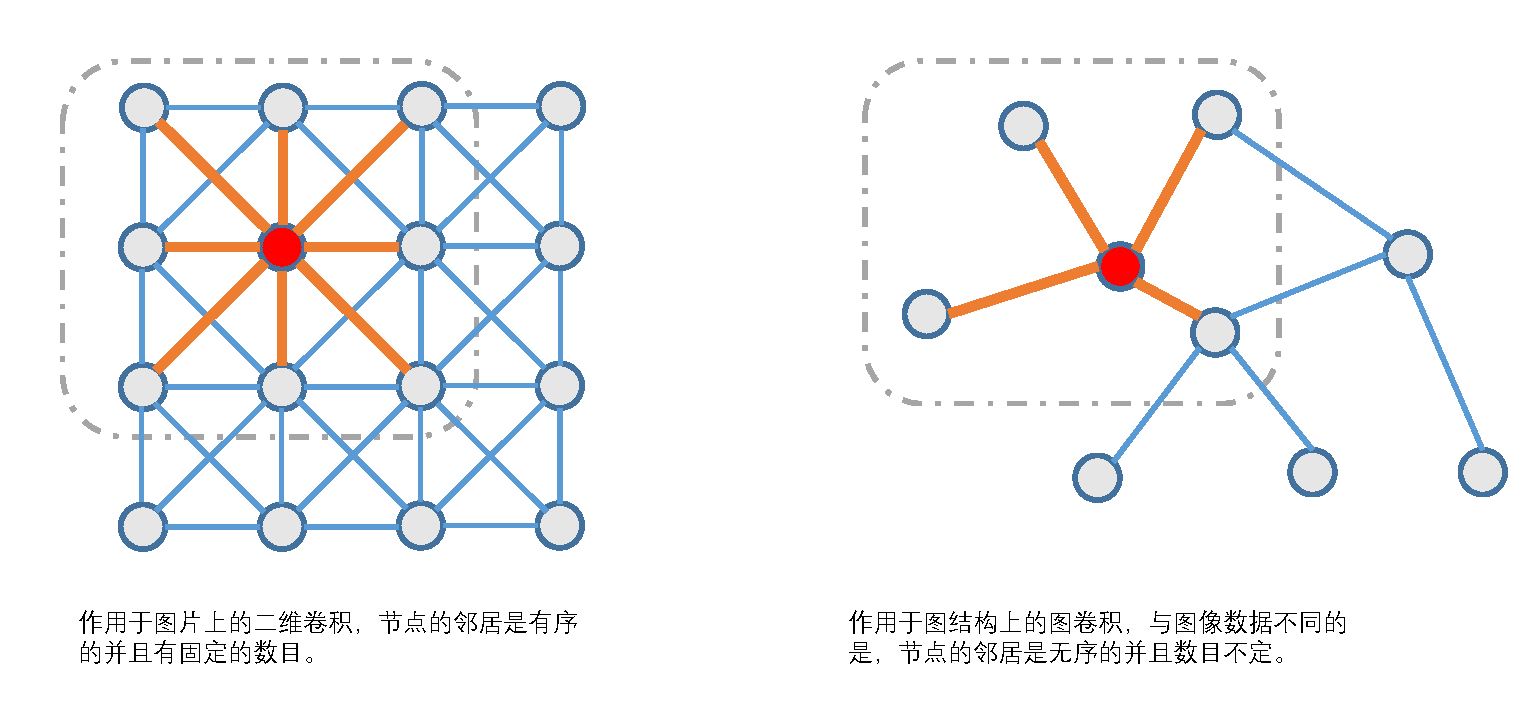
\includegraphics[width=0.9\textwidth]{fig/GCN.pdf}
    \caption{图卷积示意图}
    \label{fig:GCN}
  \end{figure}
根据卷积操作定义的不同,图卷积网络主要可以分类两类:基于谱(spectral-based)和基于空间(spatial-based)的方法。
基于谱的图卷积网络从信号处理的角度引入滤波器来定义图卷积操作,在这种方式下,图卷积操作可以看作是一种降噪操作。

基于空间的图卷积操作则是受启发于深度学习中的卷积神经网络对图像的卷积操作,与之不同的是基于空间的图卷积网络是使用图中节点之间的位置关系来进行图卷积操作的。

\subsection{图注意力网络}

图注意力网络是将注意力机制引入到基于空间域的图神经网络。图神经网络不需要使用拉普拉斯等矩阵进行复杂的计算,仅通过邻居节点的表征来更新目标节点的特征。由于能够放大数据中最重要部分的影响,注意力机制已经广泛应用到很多基于序列的任务中,图神经网络也受益于此,在聚合过程中使用注意力整合多个模型的输出。主要方法包括:
\begin{figure}[htb]
    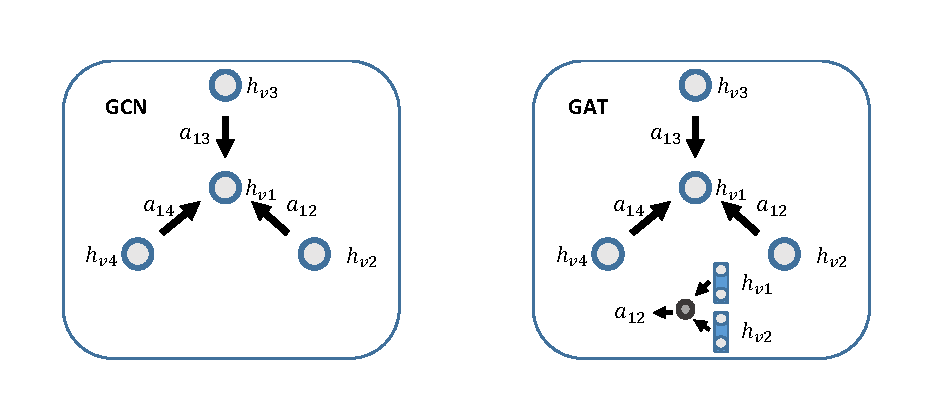
\includegraphics[width=0.9\textwidth]{fig/gcn-gat.pdf}
    \caption{GCN与GAT聚合信息的区别示意图}
    \label{fig:GCN-GAT}
  \end{figure}
\begin{itemize}
    \item Graph Attention Network(GAT)\cite{velivckovic2017graph}:本质上GAT是一种基于空间的图卷积网络,它与GCN的主要区别在于对邻居节点信息的聚合方式不同(\autoref{fig:GCN-GAT})。GCN在在聚合过程中显式地为节点$v_i$的邻居$v_j$赋予一个非参数静态权重$a_{ij}=\frac{1}{\sqrt{\operatorname{deg}\left(v_{i}\right) \operatorname{deg}\left(v_{j}\right)}}$。
    而GAT则是通过使用一个端到端的神经网络架构隐式地捕捉权重$a_{ij}$,以便更重要的节点获得更大的权重,具体操作如下:
    \begin{align}
        \mathbf{h}_{i}^{t}=\sigma\left(\sum_{j \in \mathcal{N}_{i}} \alpha\left(\mathbf{h}_{i}^{t-1}, \mathbf{h}_{j}^{t-1}\right) \mathbf{W}^{t-1} \mathbf{h}_{j}^{t-1}\right),
    \end{align}
    其中$\alpha(\cdot)$是一个注意力函数,它可以动态地调整邻居节点$j$对目标节点$i$的贡献。通常为了学习不同子空间中的注意力权重,GAT会使用多个注意力函数(即多头注意立机制,Multi-head Attention):
    \begin{align}
        \mathbf{h}_{i}^{t}=\|_{k=1}^{K} \sigma\left(\sum_{j \in \mathcal{N}_{t}} \alpha_{k}\left(\mathbf{h}_{i}^{t-1}, \mathbf{h}_{j}^{t-1}\right) W_{k}^{t-1} \mathbf{h}_{j}^{t-1}\right),
    \end{align}

    \item Gated Attention Network(GAAN)\cite{lee2017deep}\cite{zhang2018gaan}:GAAN除了采用多头注意力机制(self-attention mechanism)外,还引入了自注意机制来更新节点的隐藏状态。自注意机制可以为每个注意力头计算出一个额外的注意分数:
    \begin{align}
        \mathbf{h}_{i}^{t}=\phi_{o}\left(\mathbf{x}_{i} \oplus \|_{k=1}^{K} g_{i}^{k} \sum_{j \in \mathcal{N}_{\mathbf{t}}} \alpha_{k}\left(\mathbf{h}_{i}^{t-1}, \mathbf{h}_{j}^{t-1}\right) \phi_{v}\left(\mathbf{h}_{j}^{t-1}\right)\right),
    \end{align}
    其中$\phi_{o}\text{和}\phi_{v}$是反馈神经网络,而$g_{i}^{k}$是第$k$个注意力头的权重。
    GAM是一种基于循环神经网络模型的图神经网络,它主要应用于图数据的分类任务,即输入一个图结构数据,输出这个图所属的类别。这种方法会以自适应的方式逐个处理图中重要节点,并根据以下方式计算这些节点潜在特征:
    \begin{align}
        \mathbf{h}_{t}=\mathbf{f}_{h}\left(\mathbf{f}_{s}\left(\mathbf{r}_{t-1}, \mathbf{v}_{t-1}, g ; \theta_{s}\right), \mathbf{h}_{t-1} ; \theta_{h}\right),
    \end{align}
    其中$\mathbf{f}_{h}(\cdot)$是循环神经网络模型,通常使用LSTM,$f_s$是一个步进网络(Step Network),他会优先聚合当前节点$v_{t-1}$的邻居节点中优先级高的节点信息。
\end{itemize}
\subsection{图自编码器}
图自编码器是一类图嵌入方法,其目的是利用神经网络将图的顶点表示为低维向量。典型的解决方案是利用多层感知机作为编码器来获取节点嵌入,其中解码器重建节点的邻域统计信息,如PPMI(Positive Pointwise Mutual Information)或一阶和二阶近似值。
主要包括基于GCN的自编码器,如Graph Autoencoder(GAE)\cite{kipf2016variational}和Adversarially Regularized Graph Autoencoder (ARGA)\cite{pan2018adversarially},以及Network Representations with Adversarially Regularized Autoencoders (NetRA)\cite{yu2018learning}、Deep Neural Networks for Graph Representations (DNGR)\cite{cao2016deep}、Structural Deep Network Embedding (SDNE)\cite{wang2016structural}和Deep Recursive Network Embedding (DRNE)\cite{tu2018deep}。
DNGR和SDNE学习仅给出拓扑结构的节点嵌入,而GAE、ARGA、NetRA、DRNE用于学习当拓扑信息和节点内容特征都存在时的节点嵌入。图自动编码器的一个挑战是邻接矩阵A的稀疏性,这使得解码器的正条目数远远小于负条目数。为了解决这个问题,DNGR重构了一个更密集的矩阵,即PPMI矩阵,SDNE对邻接矩阵的零项进行惩罚,GAE对邻接矩阵中的项进行重加权,NetRA将图线性化为序列。
\subsection{图生成网络}
图生成网络的目标是在给定一组观察到的图的情况下生成新的图。图生成网络的许多方法都是特定于领域的。例如,在分子图生成中,一些工作模拟了称为SMILES的分子图的字符串表示。在自然语言处理中,生成语义图或知识图通常以给定的句子为条件。这种方法通常使用GCN或者其他框架作为基础构建模块,其中使用GCN构建的方法有:
\begin{itemize}
    \item Molecular Generative Adversarial Networks (MolGAN)\cite{de2018molgan}:MolGAN整合了图卷积网络、图注意力网络和强化学习以生成具有预期属性的图。MolGAN由生成器和判别器组成,相互竞争以提高生成器的真实性。在MolGAN中,生成器尝试提出一个假图及其特征矩阵,而鉴别器旨在将假样本与经验数据区分开来。此外,还引入了一个奖励网络来促使生成器能够按照外部的评估生成具有特定属性的图。
    \item Deep Generative Models of Graphs (DGMG)\cite{li2018learning}:利用基于空间的图卷积网络来获得现有图的隐藏表示。生成节点和边的决策过程是以整个图的表示为基础的。简而言之,DGMG递归地在一个图中产生一个节点,直到达到某个停止条件。在添加新节点后的每一步,DGMG都会反复决定是否向添加的节点添加边,直到决策的判定结果变为假。如果决策为真,则评估将新添加节点连接到所有现有节点的概率分布,并从概率分布中抽取一个节点。将新节点及其边添加到现有图形后,DGMG将更新图的表示。
\end{itemize}
使用其他架构作为基础模块的图生成网络有:
\begin{itemize}
    \item GraphRNN\cite{2018GraphRNN}:通过两个层次的循环神经网络(Recurrent Neural Network, RNN)的深度图生成模型。图层次的RNN每次向节点序列添加一个新节点,而边层次RNN生成一个二进制序列,指示新添加的节点与序列中以前生成的节点之间的连接。为了将一个图线性化为一系列节点来训练图层次的RNN,GraphRNN采用了广度优先搜索(BFS)策略。为了建立训练边层次的RNN的二元序列模型,GraphRNN假定序列服从多元伯努利分布或条件伯努利分布。
    \item NetGAN\cite{2018NetGAN}:Netgan将LSTM与Wasserstein-GAN结合在一起,使用基于随机行走的方法生成图形。GAN框架由两个模块组成,一个生成器和一个鉴别器。生成器尽最大努力在LSTM网络中生成合理的随机行走序列,而鉴别器则试图区分伪造的随机行走序列和真实的随机行走序列。训练完成后,对一组随机行走中节点的共现矩阵进行正则化,我们可以得到一个新的图。
\end{itemize}

\subsection{图时空网络}
在现实生活中,很多应用场景下的图数据都是动态的,包括拓扑结构以及特征属性。而图时空网络就是一种能够有效的处理动态图数据的模型。图时空网络的方法分为两类,一种是基于RNN的方法,另一种是基于CNN的方法。

大多数基于 RNN 的方法通过过滤输入和使用图卷积传递给循环单元的隐藏状态来捕获时空依赖性。但是基于RNN的方法存在耗时的迭代传播和梯度爆炸或者消失的问题。作为替代解决方案,基于CNN的方法以非递归的方式处理空间-时间图,具有并行计算、稳定梯度和低内存需求的优势。基于CNN的方法将一维卷积层和图卷积层交织在一起,分别学习时间和空间的依赖关系。

\subsection{任务分类}
以图结构和节点特征信息作为输入,根据输出的类别,可以将GNN的分析任务分为以下几类:
\begin{itemize}
\item 节点级别:节点级的输出与节点回归(Node Regression)和节点分类(Node Classification)任务相关。如图卷积网络可以通过信息传播和图卷积操作提取出节点的潜在表示。使用多感知器或 softmax 层作为输出层,GNN 能够以端到端的方式执行节点级任务。
\item 边级别:边级别的输出与边分类(edge classification)和链接预测(link prediction)任务相关。以GNN的两个节点的潜在表示作为输入,可以利用相似性函数或神经网络来预测一个边的标签或者连接强度。
\item 图级别:图级别的输出与图分类任务相关。通常GNN会与池化(pooling)和读出(read-out)操作相结合,以获得在图级别上的紧凑表示。
\end{itemize}

\section{本章小结}
本章总结了交通信号控制中的一些一本定义以及一些传统的交通信号控制方法,然后介绍了基于深度强化学习的智能交通信号调度的技术背景,包括强化学习、不同场景下的控制框架以及图神经网络。
